\chapter{Process}\label{chap:process}
The following chapter describes the processes used in the design and
implementation of the project. Section~\ref{sec:development-process}
provides and explanation of the development process and the approach
to implementation, and Section~\ref{sec:design-process} describes the
user-centred aspects of the design process.

\section{Development process}\label{sec:development-process}

% AGILE

\cite{martin2003agile, highsmith2001agile}

% OPENUP

\cite{balduino2007introduction, kroll2006agility}

% Project Plan Recap

\subsection{Open Source}\label{subsec:open-source}
One of the key considerations of the project objectives
(Section~\ref{sec:objectives}) was that the finished project should be
freely available without commercial interest, and this extends to the
source code and development process. The success of truly open models
of development have written about in great detail
\cite{weber2004success, godfrey2000evolution, chesbrough2006open,
  von2005democratizing}, and a philosophy of ``release early, release
often'' has been developed in open source communities as a technique
for encouraging rapid and widespread user involvement from an early
stage \cite{raymond1999cathedral}.

As a result, all of the program code, documentation and other files
that have been created for pip-db have been released under the terms
of the GNU General Public License v3 \cite{gnu2007gpl}. This is an
open and permissive license that allows for commercial use, but it
mandates that derivative works maintain the same license and must
distribute the source code openly.


\subsubsection*{A note on dataset confidentiality}
It is important to distinguish that while pip-db is an open source
project, the PIP-DB dataset as supplied by Dr.\ Flower remains
confidential, and so at his request, has not been released for
distribution.


\subsection{Version Control}\label{subsec:version-control}


% GITHUB
\cite{finley2011github}


%%%%%%%%%%%%%%%%%%%%%%%%%%%%
%% Figure: github-project %%
%%%%%%%%%%%%%%%%%%%%%%%%%%%%
\begin{figure}[H]
\centering
    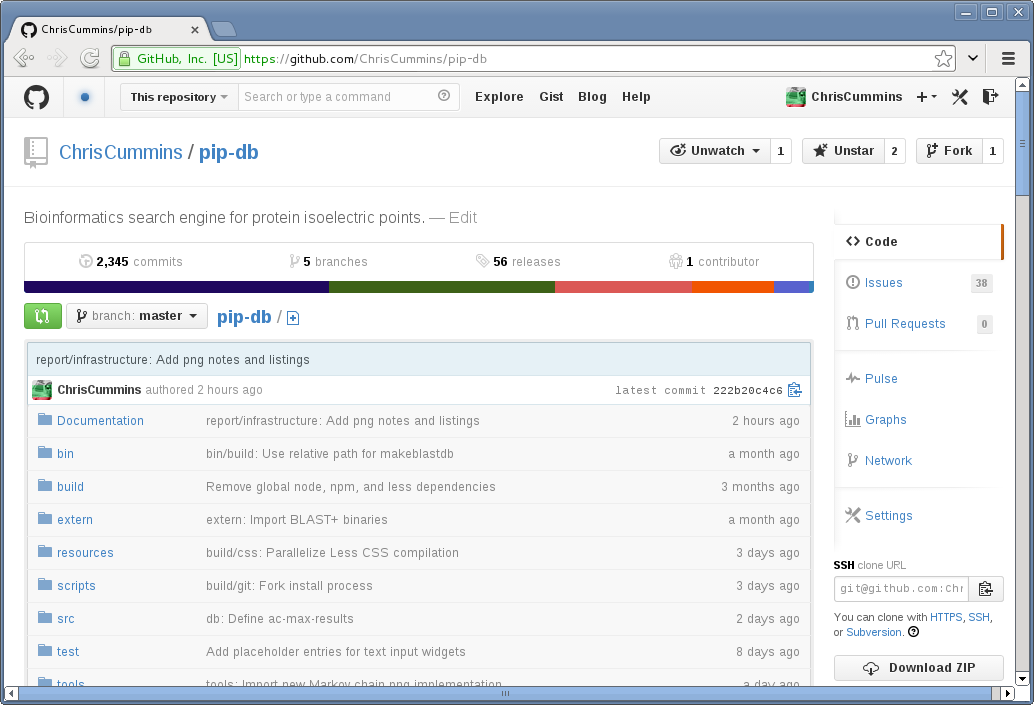
\includegraphics[width=\textwidth]{assets/github}
\caption[GitHub project homepage]
        {GitHub project homepage.}
\label{fig:github-project}
\end{figure}


\subsubsection{Branching model}

\cite{driessen2012successful}

\subsection{GitHub workflow}\label{subsec:github-workflow}

% TODO: novel workflow

% emacs + git + github = editor + version control + issue tracker

% TODO: Issue tracker


%%%%%%%%%%%%%%%%%%%%%%%%%%%
%% Figure: github-issues %%
%%%%%%%%%%%%%%%%%%%%%%%%%%%
\begin{figure}[H]
\centering
    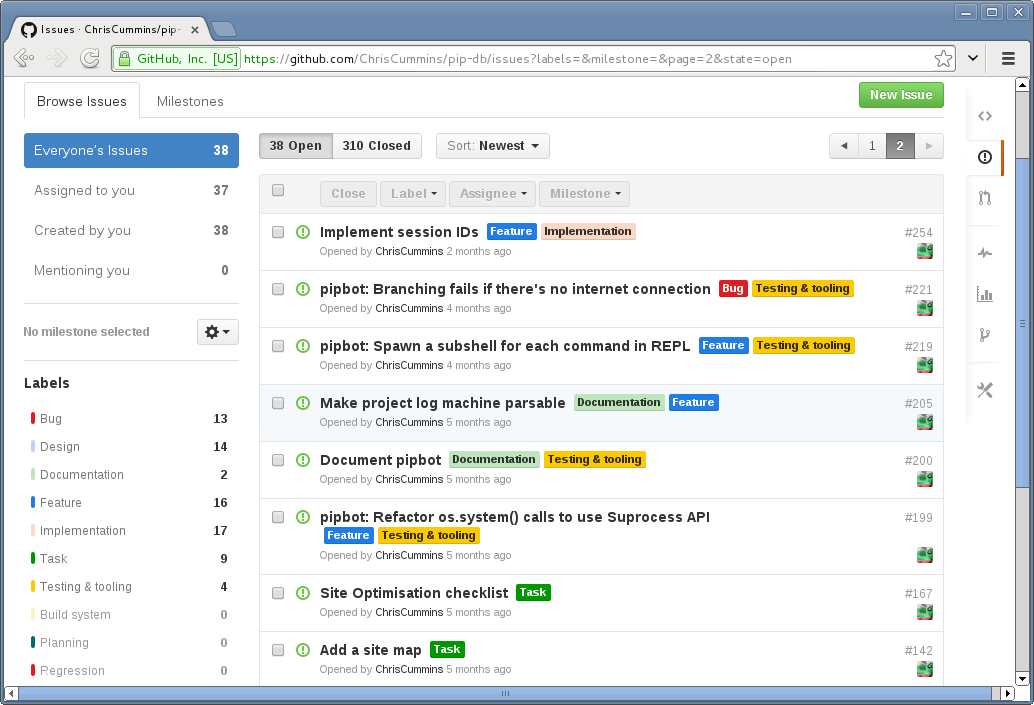
\includegraphics[width=\textwidth]{assets/github-issues}
\caption[GitHub project open issues]
        {GitHub project open issues.}
\label{fig:github-issues}
\end{figure}


% TODO: Milestones


%%%%%%%%%%%%%%%%%%%%%%%%%%%%%%%
%% Figure: github-milestones %%
%%%%%%%%%%%%%%%%%%%%%%%%%%%%%%%
\begin{figure}[H]
\centering
    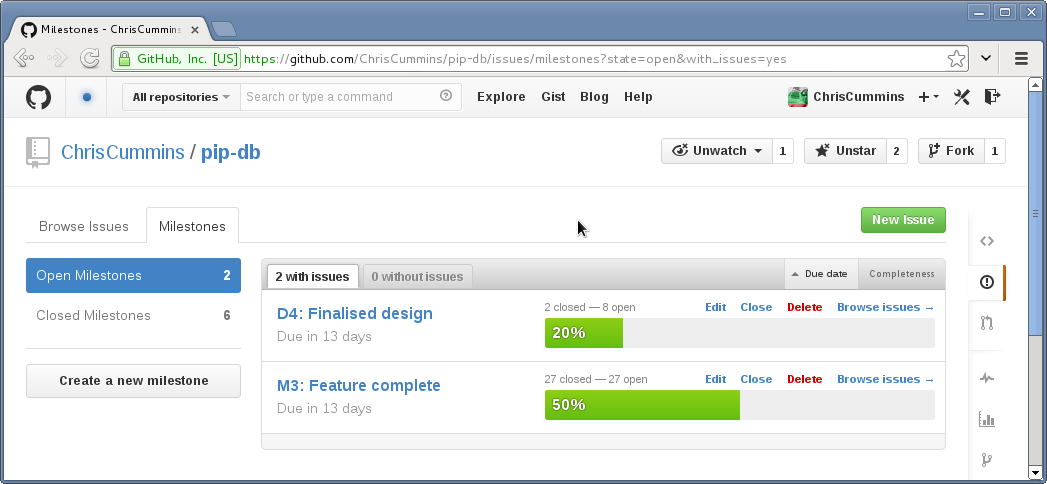
\includegraphics[width=\textwidth]{assets/github-milestones}
\caption[GitHub project open milestones]
        {GitHub project open milestones.}
\label{fig:github-milestones}
\end{figure}


\section{Design process}\label{sec:design-process}


\subsection{User-centred design}\label{subsec:user-centred-design}

% Existing systems

\cite{lu2011pubmed, hearst2007biotext}

% CRITIQUE of Darren's systems

% Usability research

\cite{bolchini2009better, pavelin2012bioinformatics}


\subsection{Low fidelity prototyping}\label{subsec:low-fidelity-prototype}

% TODO: Low-fi
\cite{egger2000lofi}

% TODO: Balsamiq


\subsection{High fidelity prototyping}\label{subsec:high-fidelity-prototype}

% TODO: Rapid prototyping using PHP + CSS + HTML + JS

% TODO: Both DESIGN and TECHNICAL prototype
